\begin{enumerate}[label=\thesection.\arabic*,ref=\thesection.\theenumi]
		\item Find $\abs{\overrightarrow{a}\times\overrightarrow{b}},\text{ if }\overrightarrow{a}=\hat{i}-7\hat{j}+7\hat{k}\text{ and } \overrightarrow{b}=3\hat{i}-2\hat{j}+2\hat{k}$.
\item Find a unit vector perpendicular to each of the vector $\overrightarrow{a}+\overrightarrow{b}\text{ and }\overrightarrow{a}-\overrightarrow{b},\text{ where } \overrightarrow{a}=3\hat{i}+2\hat{j}+2\hat{k}\text{ and } \overrightarrow{b}=\hat{i}+2\hat{j}-2\hat{k}$. 
\item If a unit vector $\overrightarrow{a}$ makes angles $\dfrac{\pi}{3}\text{ with }\hat{i}, \dfrac{\pi}{4}\text{ with }\hat{j}$ and an acute angle $\theta \text{ with }\hat{k},\text{ then find } \theta$ and hence, the components of $\overrightarrow{a}$.
	\\
		\solution
		\iffalse
\documentclass[12pt]{article}
\usepackage{graphicx}
%\documentclass[journal,12pt,twocolumn]{IEEEtran}
\usepackage[none]{hyphenat}
\usepackage{graphicx}
\usepackage{listings}
\usepackage[english]{babel}
\usepackage{graphicx}
\usepackage{caption}
\usepackage[parfill]{parskip}
\usepackage{hyperref}
\usepackage{booktabs}
\usepackage{gensymb}
%\usepackage{setspace}\doublespacing\pagestyle{plain}
\def\inputGnumericTable{}
\usepackage{color}                                            %%
    \usepackage{array}                                            %%
    \usepackage{longtable}                                        %%
    \usepackage{calc}                                             %%
    \usepackage{multirow}                                         %%
    \usepackage{hhline}                                           %%
    \usepackage{ifthen}
\usepackage{array}
\usepackage{amsmath}   % for having text in math mode
\usepackage{parallel,enumitem}
\usepackage{listings}
\lstset{
language=tex,
frame=single,
breaklines=true
}
 
%Following 2 lines were added to remove the blank page at the beginning
\usepackage{atbegshi}% http://ctan.org/pkg/atbegshi
\AtBeginDocument{\AtBeginShipoutNext{\AtBeginShipoutDiscard}}
%
%New macro definitions
\newcommand{\mydet}[1]{\ensuremath{\begin{vmatrix}#1\end{vmatrix}}}
\providecommand{\brak}[1]{\ensuremath{\left(#1\right)}}
\providecommand{\norm}[1]{\left\lVert#1\right\rVert}
\newcommand{\solution}{\noindent \textbf{Solution: }}
\newcommand{\myvec}[1]{\ensuremath{\begin{pmatrix}#1\end{pmatrix}}}
\let\vec\mathbf
\begin{document}
\begin{center}
\enlargethispage{-4cm}
\title{\textbf{Vector Algebra}}
\date{\vspace{-5ex}} %Not to print date automatically
\maketitle
\end{center}
\setcounter{page}{1}
\section*{12$^{th}$ Maths - Chapter 10}
This is Problem-3 from Exercise 10.4
\begin{enumerate}
\item If unit vector $\overrightarrow{a}$ makes angles $\frac{\pi}{3}$ with $\hat{i}$, $\frac{\pi}{4}$ with $\hat{j}$ and an acute angle $\theta$ with $\hat{k}$, then find $\theta$ and hence, the components of $\overrightarrow{a}$.

\solution
\fi
		Let 
		\begin{align}
			\vec{A}=\myvec{\cos\theta_1\\\cos\theta_2\\\cos\theta_3}
		\end{align}
		where
		\begin{align}
		\cos\theta_1 &=\cos\frac{\pi}{3}
			=\frac{1}{2}\\
			\cos\theta_2 &=\cos\frac{\pi}{4}\\
			=\frac{1}{\sqrt{2}}
		\end{align}
		Since
\begin{align}
    \norm{\vec{A}}&=1,
\sqrt{\cos^2\theta_1+\cos^2\theta_2+\cos^2\theta_3}&=1
    \implies\sqrt{\frac{1}{2}^2+\frac{1}{\sqrt{2}}^2+\cos^2\theta_3 }&=1\\
    \implies\cos\theta_3 &=\pm\frac{1}{2}
\end{align}
Since $\theta_3$ is an acute angle
\begin{align}
 \cos\theta_3=\frac{1}{2}
\end{align}
    Hence 
\begin{align}
		\vec{A}=\myvec{\frac{1}{2}\\[2pt] \frac{1}{\sqrt{2}}\\[2pt] \frac{1}{2}}
\end{align}

\item Show that $$(\overrightarrow{a}-\overrightarrow{b})\times (\overrightarrow{a}+\overrightarrow{b})=2(\overrightarrow{a}\times \overrightarrow{b})$$
\item Find $\lambda$ and $\mu$ if $(2\hat{i}+6\hat{j}+27\hat{k})\times(\hat{i}+\lambda \hat{j} + \mu \hat{k})=\overrightarrow{0}$.
	\\
		\solution
		\iffalse
\documentclass[12pt]{article}
\usepackage{graphicx}
\usepackage{amsmath}
\usepackage{mathtools}
\usepackage{gensymb}

\newcommand{\mydet}[1]{\ensuremath{\begin{vmatrix}#1\end{vmatrix}}}
\providecommand{\brak}[1]{\ensuremath{\left(#1\right)}}
\providecommand{\norm}[1]{\left\lVert#1\right\rVert}
\newcommand{\solution}{\noindent \textbf{Solution: }}
\newcommand{\myvec}[1]{\ensuremath{\begin{pmatrix}#1\end{pmatrix}}}
\let\vec\mathbf

\begin{document}
\begin{center}
\textbf\large{CHAPTER-10 \\ VECTOR ALGEBRA}

\end{center}
\section*{Excercise 10.4}

Q5.Find $\lambda \text{ and } \mu \text{ if } (2\hat{i}+6\hat{j}+27\hat{k}) \times (\hat{i}+\lambda \hat{j}+\mu \hat{k})=\vec{0}$

\solution
\fi
\begin{align}
	\text{Let } \vec{A} = \myvec{2\\6\\27} \text{ and } \vec{B} = \myvec{1\\ \lambda \\ \mu}\\
\end{align}
The cross product or vector product of $\vec{A},\vec{B}$ is defined as
\begin{align}
	\vec{A} \times \vec{B} = \myvec{\mydet{\vec{A}_{23}&\vec{B}_{23}\\\vec{A}_{31}&\vec{B}_{31}\\\vec{A}_{12}&\vec{B}_{12}}}
\end{align}
Hence
\begin{align}
	\mydet{\vec{A}_{23}&\vec{B}_{23}}&=\mydet{6&\lambda\\27&\mu}=6\mu-27\lambda\\
	\mydet{\vec{A}_{31}&\vec{B}_{31}}&=\mydet{27&\mu\\2&1}=27-2\mu\\
	\mydet{\vec{A}_{12}&\vec{B}_{12}}&=\mydet{2&1\\6&\lambda}=2\lambda-6
\end{align}
Substituting the values
\begin{align}
	\vec{A}\times\vec{B}=\myvec{6\mu-27\lambda\\27-2\mu\\2\lambda-6}
\end{align}
Since
\begin{align}
	\vec{A} \times \vec{B} &= \vec{0},
	\\
	\myvec{6\mu-27\lambda\\27-2\mu\\2\lambda-6}&=\myvec{0\\0\\0},
\end{align}
which can be represented in matrix form as
\begin{align}
	\myvec{2&0\\0&2\\6&-27}\myvec{\mu\\\lambda}&=\myvec{27\\6\\0}.
\end{align}
The augmented matrix is given as
\begin{align}
	\myvec{2 & 0 & \vrule & 27\\0 & 2 & \vrule & 6\\ 6 & -27 & \vrule & 0}
	\xleftrightarrow{R_{3}\rightarrow R_{3}-3R_{1}}  	
	\myvec{2 & 0 & \vrule & 27\\0 & 2 & \vrule & 6\\ 0 & -27 & \vrule & -81}\\
	\xleftrightarrow{R_{3}\rightarrow R_{3}+\frac{27}{2}R_{2}}  	
	\myvec{2 & 0 & \vrule & 27\\0 & 2 & \vrule & 6\\ 0 & 0 & \vrule & 0}
\end{align}
yielding
\begin{align}
	\mu=13.5,
	\lambda=3
\end{align}


\item Given that $\overrightarrow{a} \cdot \overrightarrow{b} = 0$ and $\overrightarrow{a} \times \overrightarrow{b} = \overrightarrow{0}$. What can you conclude about the vectors $\overrightarrow{a} \text{ and }\overrightarrow{b}$?
\item Let the vectors be given as $\overrightarrow{a},\overrightarrow{b},\overrightarrow{c}\text{ be given as }\ a_1 \hat{i}+\ a_2 \hat{j}+\ a_3 \hat{k},\ b_1 \hat{i}+\ b_2 \hat{j}+\ b_3 \hat{k},\ c_1 \hat{i}+\ c_2 \hat{j}+\ c_3 \hat{k}$. Then show that $\overrightarrow{a} \times (\overrightarrow{b} + \overrightarrow{c}) = \overrightarrow{a} \times \overrightarrow{b}+\overrightarrow{a} \times \overrightarrow{c}$.
	\\
		\solution
		\iffalse
\documentclass[A4,12pt,twocolumn]{IEEEtran}
%
\usepackage{setspace}
\usepackage{gensymb}
%\doublespacing
\singlespacing

%\usepackage{graphicx}
%\usepackage{amssymb}
%\usepackage{relsize}
\usepackage[cmex10]{amsmath}
%\usepackage{amsthm}
%\interdisplaylinepenalty=2500
%\savesymbol{iint}
%\usepackage{txfonts}
%\restoresymbol{TXF}{iint}
%\usepackage{wasysym}
\usepackage{amsthm}
%\usepackage{iithtlc}
\usepackage{mathrsfs}
\usepackage{txfonts}
\usepackage{stfloats}
\usepackage{bm}
\usepackage{cite}
\usepackage{cases}
\usepackage{subfig}
%\usepackage{xtab}
\usepackage{longtable}
\usepackage{multirow}
%\usepackage{algorithm}
%\usepackage{algpseudocode}
\usepackage{enumitem}
\usepackage{mathtools}
\usepackage{steinmetz}
\usepackage{tikz}
\usepackage{circuitikz}
\usepackage{verbatim}
\usepackage{tfrupee}
\usepackage[breaklinks=true]{hyperref}
%\usepackage{stmaryrd}
\usepackage{tkz-euclide} % loads  TikZ and tkz-base
%\usetkzobj{all}
\usetikzlibrary{calc,math}
\usepackage{listings}
    \usepackage{color}                                            %%
    \usepackage{array}                                            %%
    \usepackage{longtable}                                        %%
    \usepackage{calc}                                             %%
    \usepackage{multirow}                                         %%
    \usepackage{hhline}                                           %%
    \usepackage{ifthen}                                           %%
  %optionally (for landscape tables embedded in another document): %%
    \usepackage{lscape}     
\usepackage{multicol}
\usepackage{chngcntr}
%\usepackage{enumerate}

%\usepackage{wasysym}
%\newcounter{MYtempeqncnt}
\DeclareMathOperator*{\Res}{Res}
%\renewcommand{\baselinestretch}{2}
\renewcommand\thesection{\arabic{section}}
\renewcommand\thesubsection{\thesection.\arabic{subsection}}
\renewcommand\thesubsubsection{\thesubsection.\arabic{subsubsection}}

\renewcommand\thesectiondis{\arabic{section}}
\renewcommand\thesubsectiondis{\thesectiondis.\arabic{subsection}}
\renewcommand\thesubsubsectiondis{\thesubsectiondis.\arabic{subsubsection}}

% correct bad hyphenation here
\hyphenation{op-tical net-works semi-conduc-tor}
\def\inputGnumericTable{}                                 %%

\lstset{
%language=C,
frame=single, 
breaklines=true,
columns=fullflexible
}
%\lstset{
%language=tex,
%frame=single, 
%breaklines=true
%}

\begin{document}
%


\newtheorem{theorem}{Theorem}[section]
\newtheorem{problem}{Problem}
\newtheorem{proposition}{Proposition}[section]
\newtheorem{lemma}{Lemma}[section]
\newtheorem{corollary}[theorem]{Corollary}
\newtheorem{example}{Example}[section]
\newtheorem{definition}[problem]{Definition}
%\newtheorem{thm}{Theorem}[section] 
%\newtheorem{defn}[thm]{Definition}
%\newtheorem{algorithm}{Algorithm}[section]
%\newtheorem{cor}{Corollary}
\newcommand{\BEQA}{\begin{eqnarray}}
\newcommand{\EEQA}{\end{eqnarray}}
\newcommand{\define}{\stackrel{\triangle}{=}}

\bibliographystyle{IEEEtran}
%\bibliographystyle{ieeetr}


\providecommand{\mbf}{\mathbf}
\providecommand{\pr}[1]{\ensuremath{\Pr\left(#1\right)}}
\providecommand{\qfunc}[1]{\ensuremath{Q\left(#1\right)}}
\providecommand{\sbrak}[1]{\ensuremath{{}\left[#1\right]}}
\providecommand{\lsbrak}[1]{\ensuremath{{}\left[#1\right.}}
\providecommand{\rsbrak}[1]{\ensuremath{{}\left.#1\right]}}
\providecommand{\brak}[1]{\ensuremath{\left(#1\right)}}
\providecommand{\lbrak}[1]{\ensuremath{\left(#1\right.}}
\providecommand{\rbrak}[1]{\ensuremath{\left.#1\right)}}
\providecommand{\cbrak}[1]{\ensuremath{\left\{#1\right\}}}
\providecommand{\lcbrak}[1]{\ensuremath{\left\{#1\right.}}
\providecommand{\rcbrak}[1]{\ensuremath{\left.#1\right\}}}
\theoremstyle{remark}
\newtheorem{rem}{Remark}
\newcommand{\sgn}{\mathop{\mathrm{sgn}}}
\providecommand{\abs}[1]{\left\vert#1\right\vert}
\providecommand{\res}[1]{\Res\displaylimits_{#1}} 
\providecommand{\norm}[1]{\left\lVert#1\right\rVert}
%\providecommand{\norm}[1]{\lVert#1\rVert}
\providecommand{\mtx}[1]{\mathbf{#1}}
\providecommand{\mean}[1]{E\left[ #1 \right]}
\providecommand{\fourier}{\overset{\mathcal{F}}{ \rightleftharpoons}}
%\providecommand{\hilbert}{\overset{\mathcal{H}}{ \rightleftharpoons}}
\providecommand{\system}{\overset{\mathcal{H}}{ \longleftrightarrow}}
	%\newcommand{\solution}[2]{\textbf{Solution:}{#1}}
\newcommand{\solution}{\noindent \textbf{Solution: }}
\newcommand{\cosec}{\,\text{cosec}\,}
\providecommand{\dec}[2]{\ensuremath{\overset{#1}{\underset{#2}{\gtrless}}}}
\newcommand{\myvec}[1]{\ensuremath{\begin{pmatrix}#1\end{pmatrix}}}
\newcommand{\mydet}[1]{\ensuremath{\begin{vmatrix}#1\end{vmatrix}}}
%\numberwithin{equation}{section}
\numberwithin{equation}{subsection}
%\numberwithin{problem}{section}
%\numberwithin{definition}{section}
\makeatletter
\@addtoreset{figure}{problem}
\makeatother

\let\StandardTheFigure\thefigure
\let\vec\mathbf
%\renewcommand{\thefigure}{\theproblem.\arabic{figure}}
\renewcommand{\thefigure}{\theproblem}
%\setlist[enumerate,1]{before=\renewcommand\theequation{\theenumi.\arabic{equation}}
%\counterwithin{equation}{enumi}


%\renewcommand{\theequation}{\arabic{subsection}.\arabic{equation}}

\def\putbox#1#2#3{\makebox[0in][l]{\makebox[#1][l]{}\raisebox{\baselineskip}[0in][0in]{\raisebox{#2}[0in][0in]{#3}}}}
     \def\rightbox#1{\makebox[0in][r]{#1}}
     \def\centbox#1{\makebox[0in]{#1}}
     \def\topbox#1{\raisebox{-\baselineskip}[0in][0in]{#1}}
     \def\midbox#1{\raisebox{-0.5\baselineskip}[0in][0in]{#1}}

\vspace{3cm}


\title{QUIZ 4}
\author{Shristy Sharma (EE22BNITS11001)}





% make the title area
\maketitle

\newpage

%\tableofcontents

\bigskip

\renewcommand{\thefigure}{\theenumi}
\renewcommand{\thetable}{\theenumi}
%\renewcommand{\theequation}{\theenumi}


%Download all python codes 
%
%\begin{lstlisting}
%svn co https://github.com/JayatiD93/trunk/My_solution_design/codes
%\end{lstlisting}

%Download all and latex-tikz codes from 
%
%\begin{lstlisting}
%svn co https://github.com/gadepall/school/trunk/ncert/geometry/figs
%\end{lstlisting}
%


\section{PROBLEM 1}
1. Let the vector
\begin{align}
\vec{a}=\myvec{a_1\\a_2\\a_3},
\vec{b}=\myvec{b_1\\b_2\\b_3}, 
\vec{c}=\myvec{c_1\\c_2\\c_3}
\end{align} 
Then show that $ \vec{a} \times (\vec{b}+\vec{c})$ = $ \vec{a} \times \vec{b}+\vec{a} \times \vec{c})$ \\
\\SOLUTION:
\fi`
Let,
\begin{align}
 \vec{a}= \myvec{2\\3\\1} ,\vec{b}= \myvec{1\\2\\1}, \vec{c}= \myvec{1\\1\\1}\\
\end{align}
Then
\begin{align}
 \vec{a} \times ({\vec{b}+\vec{c}}) 
&= \myvec{2\\3\\1} \times \myvec{2\\3\\2} \\
&= \myvec{3\\-2\\0} 
\end{align}
Similarly, 
\begin{align}
 (\vec{a} \times \vec{b})+(\vec{a} \times \vec{c}) 
= \myvec{1\\-1\\1} +  \myvec{2\\-1\\-1}
= \myvec{3\\-2\\0} 
\end{align}




\item If either $\overrightarrow{a} = \overrightarrow{0}$ or $\overrightarrow{b} = \overrightarrow{0}$, then $\overrightarrow{a} \times \overrightarrow{b} = \overrightarrow{0}$. Is the converse true? Justify your answer with an example.
\item Find the area of the triangle with vertices $A(1, 1, 2)$, $B(2, 3, 5)$, and $C(1, 5, 5)$
	\\
		\solution
		\iffalse
\documentclass[journal,12pt,twocolumn]{IEEEtran}
\usepackage{setspace}
\usepackage{gensymb}
\singlespacing
\usepackage[cmex10]{amsmath}
\usepackage{amsthm}
\usepackage{mathrsfs}
\usepackage{txfonts}
\usepackage{stfloats}
\usepackage{bm}
\usepackage{cite}
\usepackage{cases}
\usepackage{subfig}
\usepackage{longtable}
\usepackage{multirow}
\usepackage{enumitem}
\usepackage{mathtools}
\usepackage{steinmetz}
\usepackage{tikz}
\usepackage{circuitikz}
\usepackage{verbatim}
\usepackage{tfrupee}
\usepackage[breaklinks=true]{hyperref}
\usepackage{tkz-euclide}
\usetikzlibrary{calc,math}
\usepackage{listings}
    \usepackage{color}                                            %%
    \usepackage{array}                                            %%
    \usepackage{longtable}                                        %%
    \usepackage{calc}                                             %%
    \usepackage{multirow}                                         %%
    \usepackage{hhline}                                           %%
    \usepackage{ifthen}                                           %%
  %optionally (for landscape tables embedded in another document): %%
    \usepackage{lscape}     
\usepackage{multicol}
\usepackage{chngcntr}
\DeclareMathOperator*{\Res}{Res}
\renewcommand\thesection{\arabic{section}}
\renewcommand\thesubsection{\thesection.\arabic{subsection}}
\renewcommand\thesubsubsection{\thesubsection.\arabic{subsubsection}}

\renewcommand\thesectiondis{\arabic{section}}
\renewcommand\thesubsectiondis{\thesectiondis.\arabic{subsection}}
\renewcommand\thesubsubsectiondis{\thesubsectiondis.\arabic{subsubsection}}

% correct bad hyphenation here
\hyphenation{op-tical net-works semi-conduc-tor}
\def\inputGnumericTable{}                                 %%

\lstset{
frame=single, 
breaklines=true,
columns=fullflexible
}

\begin{document}


\newtheorem{theorem}{Theorem}[section]
\newtheorem{problem}{Problem}
\newtheorem{proposition}{Proposition}[section]
\newtheorem{lemma}{Lemma}[section]
\newtheorem{corollary}[theorem]{Corollary}
\newtheorem{example}{Example}[section]
\newtheorem{definition}[problem]{Definition}
\newcommand{\BEQA}{\begin{eqnarray}}
\newcommand{\EEQA}{\end{eqnarray}}
\newcommand{\define}{\stackrel{\triangle}{=}}

\bibliographystyle{IEEEtran}
\providecommand{\mbf}{\mathbf}
\providecommand{\pr}[1]{\ensuremath{\Pr\left(#1\right)}}
\providecommand{\qfunc}[1]{\ensuremath{Q\left(#1\right)}}
\providecommand{\sbrak}[1]{\ensuremath{{}\left[#1\right]}}
\providecommand{\lsbrak}[1]{\ensuremath{{}\left[#1\right.}}
\providecommand{\rsbrak}[1]{\ensuremath{{}\left.#1\right]}}
\providecommand{\brak}[1]{\ensuremath{\left(#1\right)}}
\providecommand{\lbrak}[1]{\ensuremath{\left(#1\right.}}
\providecommand{\rbrak}[1]{\ensuremath{\left.#1\right)}}
\providecommand{\cbrak}[1]{\ensuremath{\left\{#1\right\}}}
\providecommand{\lcbrak}[1]{\ensuremath{\left\{#1\right.}}
\providecommand{\rcbrak}[1]{\ensuremath{\left.#1\right\}}}
\theoremstyle{remark}
\newtheorem{rem}{Remark}
\newcommand{\sgn}{\mathop{\mathrm{sgn}}}
\providecommand{\abs}[1]{\left\vert#1\right\vert}
\providecommand{\res}[1]{\Res\displaylimits_{#1}} 
\providecommand{\norm}[1]{\left\lVert#1\right\rVert}
\providecommand{\mtx}[1]{\mathbf{#1}}
\providecommand{\mean}[1]{E\left[ #1 \right]}
\providecommand{\fourier}{\overset{\mathcal{F}}{ \rightleftharpoons}}
\providecommand{\system}{\overset{\mathcal{H}}{ \longleftrightarrow}}
\newcommand{\solution}{\noindent \textbf{Solution: }}
\newcommand{\cosec}{\,\text{cosec}\,}
\providecommand{\dec}[2]{\ensuremath{\overset{#1}{\underset{#2}{\gtrless}}}}
\newcommand{\myvec}[1]{\ensuremath{\begin{pmatrix}#1\end{pmatrix}}}
\newcommand{\mydet}[1]{\ensuremath{\begin{vmatrix}#1\end{vmatrix}}}
\numberwithin{equation}{subsection}
\makeatletter
\@addtoreset{figure}{problem}
\makeatother

\let\StandardTheFigure\thefigure
\let\vec\mathbf
\renewcommand{\thefigure}{\theproblem}



\def\putbox#1#2#3{\makebox[0in][l]{\makebox[#1][l]{}\raisebox{\baselineskip}[0in][0in]{\raisebox{#2}[0in][0in]{#3}}}}
     \def\rightbox#1{\makebox[0in][r]{#1}}
     \def\centbox#1{\makebox[0in]{#1}}
     \def\topbox#1{\raisebox{-\baselineskip}[0in][0in]{#1}}
     \def\midbox#1{\raisebox{-0.5\baselineskip}[0in][0in]{#1}}

\vspace{3cm}


\title{Assignment 1}
\author{Jaswanth Chowdary Madala}





% make the title area
\maketitle

\newpage

%\tableofcontents

\bigskip

\renewcommand{\thefigure}{\theenumi}
\renewcommand{\thetable}{\theenumi}

\begin{enumerate}
\item Find the area of the triangle with vertices $\vec{A}$(1,1,2), $\vec{B}$ (2,3,5), $\vec{C}$ (1,5,5).

\textbf{Solution:} The area of the triangle $ABC$ is given by
\begin{align}
ar(ABC) &= \dfrac{1}{2}\norm{\brak{\vec{B}-\vec{A}} \times \brak{\vec{C}-\vec{A}}}
\end{align}


given points are 
\fi
Since
\begin{align}
\vec{B}-\vec{A} = \myvec{1\\2\\3}, 
\vec{C}-\vec{A} = \myvec{0\\4\\3} \\
\end{align}
the desired area is given by 
\begin{align}
	\frac{1}{2} \norm{\myvec{1\\2\\3} \times \myvec{0\\4\\3}} 
	= 	\frac{1}{2}\norm{\myvec{-6\\3\\4}}
= \dfrac{\sqrt{61}}{2}
\end{align}






\item Find the area of the parallelogram whose adjacent sides are determined by the vectors $\overrightarrow{a}=\hat{i}-\hat{j}+3\hat{k}$ and $\overrightarrow{b}=2\hat{i}-7\hat{j}+\hat{k}$.
\item Let the vectors $\overrightarrow{a}$ and $\overrightarrow{b}$ be such that $|\overrightarrow{a}| = 3$ and $|\overrightarrow{b}| = \dfrac{\sqrt{2}}{3}$, then $\overrightarrow{a} \times \overrightarrow{b}$ is a unit vector, if the angle between $\overrightarrow{a}$ and $\overrightarrow{b}$ is
\begin{enumerate}
\item $\dfrac{\pi}{6}$
\item $\dfrac{\pi}{4}$
\item $\dfrac{\pi}{3}$
\item $\dfrac{\pi}{2}$
\end{enumerate}
\item Area of a rectangle having vertices A, B, C and D with position vectors $ -\hat{i}+ \dfrac{1}{2} \hat{j}+4\hat{k},\hat{i}+ \dfrac{1}{2} \hat{j}+4\hat{k},\hat{i}-\dfrac{1}{2} \hat{j}+4\hat{k}\text{ and }-\hat{i}- \dfrac{1}{2} \hat{j}+4\hat{k}$, respectively is
\begin{enumerate}
\item $\dfrac{1}{2}$
\item 1
\item 2
\item 4
\end{enumerate}
		\solution
		\iffalse
\documentclass[journal,12pt,twocolumn]{IEEEtran}
%
\usepackage{setspace}
\usepackage{gensymb}
%\doublespacing
\singlespacing

%\usepackage{graphicx}
%\usepackage{amssymb}
%\usepackage{relsize}
\usepackage[cmex10]{amsmath}
%\usepackage{amsthm}
%\interdisplaylinepenalty=2500
%\savesymbol{iint}
%\usepackage{txfonts}
%\restoresymbol{TXF}{iint}
%\usepackage{wasysym}
\usepackage{amsthm}
%\usepackage{iithtlc}
\usepackage{mathrsfs}
\usepackage{txfonts}
\usepackage{stfloats}
\usepackage{bm}
\usepackage{cite}
\usepackage{cases}
\usepackage{subfig}
%\usepackage{xtab}
\usepackage{longtable}
\usepackage{multirow}
%\usepackage{algorithm}
%\usepackage{algpseudocode}
\usepackage{enumitem}
\usepackage{mathtools}
\usepackage{steinmetz}
\usepackage{tikz}
\usepackage{circuitikz}
\usepackage{verbatim}
\usepackage{tfrupee}
\usepackage[breaklinks=true]{hyperref}
%\usepackage{stmaryrd}
\usepackage{tkz-euclide} % loads  TikZ and tkz-base
%\usetkzobj{all}
\usetikzlibrary{calc,math}
\usepackage{listings}
    \usepackage{color}                                            %%
    \usepackage{array}                                            %%
    \usepackage{longtable}                                        %%
    \usepackage{calc}                                             %%
    \usepackage{multirow}                                         %%
    \usepackage{hhline}                                           %%
    \usepackage{ifthen}                                           %%
  %optionally (for landscape tables embedded in another document): %%
    \usepackage{lscape}     
\usepackage{multicol}
\usepackage{chngcntr}
%\usepackage{enumerate}

%\usepackage{wasysym}
%\newcounter{MYtempeqncnt}
\DeclareMathOperator*{\Res}{Res}
%\renewcommand{\baselinestretch}{2}
\renewcommand\thesection{\arabic{section}}
\renewcommand\thesubsection{\thesection.\arabic{subsection}}
\renewcommand\thesubsubsection{\thesubsection.\arabic{subsubsection}}

\renewcommand\thesectiondis{\arabic{section}}
\renewcommand\thesubsectiondis{\thesectiondis.\arabic{subsection}}
\renewcommand\thesubsubsectiondis{\thesubsectiondis.\arabic{subsubsection}}

% correct bad hyphenation here
\hyphenation{op-tical net-works semi-conduc-tor}
\def\inputGnumericTable{}                                 %%

\lstset{
%language=C,
frame=single, 
breaklines=true,
columns=fullflexible
}
%\lstset{
%language=tex,
%frame=single, 
%breaklines=true
%}

\begin{document}
%


\newtheorem{theorem}{Theorem}[section]
\newtheorem{problem}{Problem}
\newtheorem{proposition}{Proposition}[section]
\newtheorem{lemma}{Lemma}[section]
\newtheorem{corollary}[theorem]{Corollary}
\newtheorem{example}{Example}[section]
\newtheorem{definition}[problem]{Definition}
%\newtheorem{thm}{Theorem}[section] 
%\newtheorem{defn}[thm]{Definition}
%\newtheorem{algorithm}{Algorithm}[section]
%\newtheorem{cor}{Corollary}
\newcommand{\BEQA}{\begin{eqnarray}}
\newcommand{\EEQA}{\end{eqnarray}}
\newcommand{\define}{\stackrel{\triangle}{=}}

\bibliographystyle{IEEEtran}
%\bibliographystyle{ieeetr}


\providecommand{\mbf}{\mathbf}
\providecommand{\pr}[1]{\ensuremath{\Pr\left(#1\right)}}
\providecommand{\qfunc}[1]{\ensuremath{Q\left(#1\right)}}
\providecommand{\sbrak}[1]{\ensuremath{{}\left[#1\right]}}
\providecommand{\lsbrak}[1]{\ensuremath{{}\left[#1\right.}}
\providecommand{\rsbrak}[1]{\ensuremath{{}\left.#1\right]}}
\providecommand{\brak}[1]{\ensuremath{\left(#1\right)}}
\providecommand{\lbrak}[1]{\ensuremath{\left(#1\right.}}
\providecommand{\rbrak}[1]{\ensuremath{\left.#1\right)}}
\providecommand{\cbrak}[1]{\ensuremath{\left\{#1\right\}}}
\providecommand{\lcbrak}[1]{\ensuremath{\left\{#1\right.}}
\providecommand{\rcbrak}[1]{\ensuremath{\left.#1\right\}}}
\theoremstyle{remark}
\newtheorem{rem}{Remark}
\newcommand{\sgn}{\mathop{\mathrm{sgn}}}
\providecommand{\abs}[1]{\left\vert#1\right\vert}
\providecommand{\res}[1]{\Res\displaylimits_{#1}} 
\providecommand{\norm}[1]{\left\lVert#1\right\rVert}
%\providecommand{\norm}[1]{\lVert#1\rVert}
\providecommand{\mtx}[1]{\mathbf{#1}}
\providecommand{\mean}[1]{E\left[ #1 \right]}
\providecommand{\fourier}{\overset{\mathcal{F}}{ \rightleftharpoons}}
%\providecommand{\hilbert}{\overset{\mathcal{H}}{ \rightleftharpoons}}
\providecommand{\system}{\overset{\mathcal{H}}{ \longleftrightarrow}}
	%\newcommand{\solution}[2]{\textbf{Solution:}{#1}}
\newcommand{\solution}{\noindent \textbf{Solution: }}
\newcommand{\cosec}{\,\text{cosec}\,}
\providecommand{\dec}[2]{\ensuremath{\overset{#1}{\underset{#2}{\gtrless}}}}
\newcommand{\myvec}[1]{\ensuremath{\begin{pmatrix}#1\end{pmatrix}}}
\newcommand{\mydet}[1]{\ensuremath{\begin{vmatrix}#1\end{vmatrix}}}
%\numberwithin{equation}{section}
\numberwithin{equation}{subsection}
%\numberwithin{problem}{section}
%\numberwithin{definition}{section}
\makeatletter
\@addtoreset{figure}{problem}
\makeatother

\let\StandardTheFigure\thefigure
\let\vec\mathbf
%\renewcommand{\thefigure}{\theproblem.\arabic{figure}}
\renewcommand{\thefigure}{\theproblem}
%\setlist[enumerate,1]{before=\renewcommand\theequation{\theenumi.\arabic{equation}}
%\counterwithin{equation}{enumi}


%\renewcommand{\theequation}{\arabic{subsection}.\arabic{equation}}

\def\putbox#1#2#3{\makebox[0in][l]{\makebox[#1][l]{}\raisebox{\baselineskip}[0in][0in]{\raisebox{#2}[0in][0in]{#3}}}}
     \def\rightbox#1{\makebox[0in][r]{#1}}
     \def\centbox#1{\makebox[0in]{#1}}
     \def\topbox#1{\raisebox{-\baselineskip}[0in][0in]{#1}}
     \def\midbox#1{\raisebox{-0.5\baselineskip}[0in][0in]{#1}}

\vspace{3cm}


\title{Question: 12.10.4.12}
\author{Nikam Pratik Balasaheb (EE21BTECH11037)}





% make the title area
\maketitle

\newpage

%\tableofcontents

\bigskip

\renewcommand{\thefigure}{\theenumi}
\renewcommand{\thetable}{\theenumi}
%\renewcommand{\theequation}{\theenumi}

\section{Problem}
Find the area of rectangle having A,B,C,D with position vectors $\myvec{-1\\[1pt]\frac{1}{2} \\[1pt] 4}$ ,$\myvec{1\\[1pt]\frac{1}{2} \\[1pt] 4}$, $\myvec{1\\[1pt]\frac{-1}{2} \\[1pt] 4}$ and $\myvec{-1\\[1pt]\frac{-1}{2} \\[1pt] 4}$ respectively.  
\section{Solution}
\fi
Since
\begin{align}
\vec{A} - \vec{B} &= \myvec{-2\\0\\0}\\
\vec{C} -\vec{B} &= \myvec{0\\-1\\0}
\end{align}
area of the rectangle is
\begin{align}
 \norm{\brak{\vec{A} -\vec{B}} \times \brak{\vec{C}-\vec{D}}}
= 2
\end{align} 
See Fig. 
   \ref{fig:chapters/12/10/4/12Rect_ABCD}
\begin{figure}[h!]
  \centering
   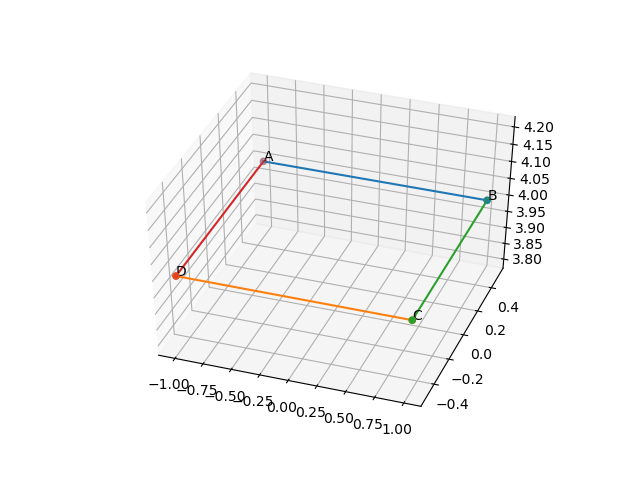
\includegraphics[width=\columnwidth]{chapters/12/10/4/12/figs/Figure_1.png}
   \caption{}
   \label{fig:chapters/12/10/4/12Rect_ABCD}
\end{figure}





\end{enumerate}

